\documentclass{article}
\usepackage[utf8]{inputenc}
\usepackage[russian]{babel}
\usepackage[left=2cm,right=2cm,
top=2cm,bottom=2cm,bindingoffset=0cm]{geometry}
\usepackage{graphicx}
\usepackage{amsmath}
\usepackage{float}
\usepackage{listings}
\usepackage{url,textcomp}
\date{2019 г.}
\author{Кондратенко Федор, гр 13632/1}
\setlength{\parindent}{0pt}
\setlength{\parskip}{5pt plus 2pt minus 1pt}
\frenchspacing
\title{Отчет по заданию №5}
\begin{document}
	\maketitle
	\subsection*{Математический маятник}
	Для имитационного моделирования математического маятника в Simscape Multibody была взята готовая модель из примеров, в которую были внесены изменения:
	\begin{figure}[H]
		\centering
		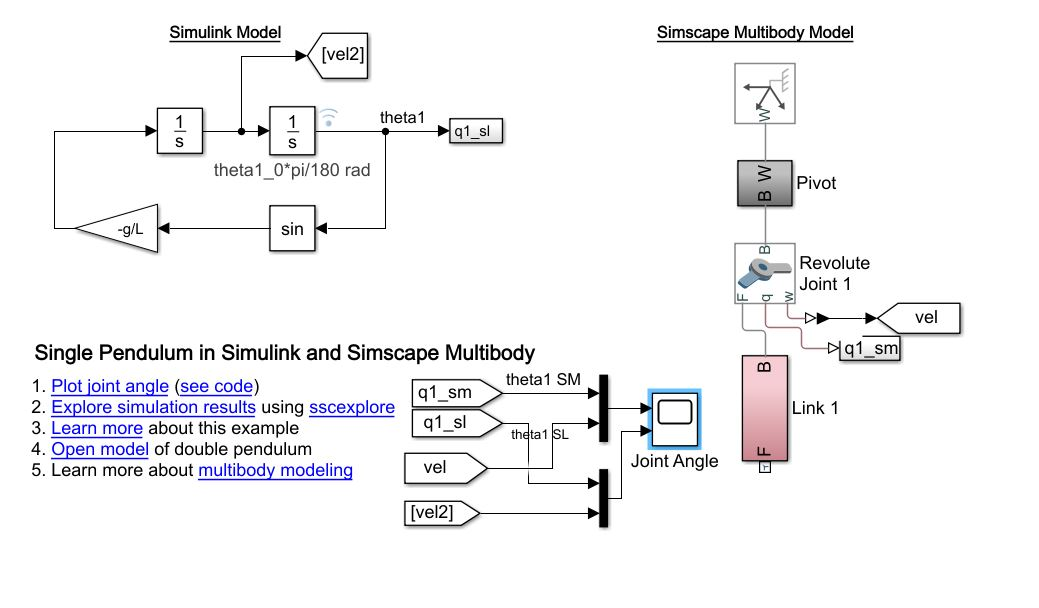
\includegraphics[width=0.7\linewidth]{model1}
		\caption{Блок-схема модели}
		\label{fig:model}
	\end{figure}
	Моделирование свободных колебаний математического маятника:
	\begin{figure}[H]
		\centering
		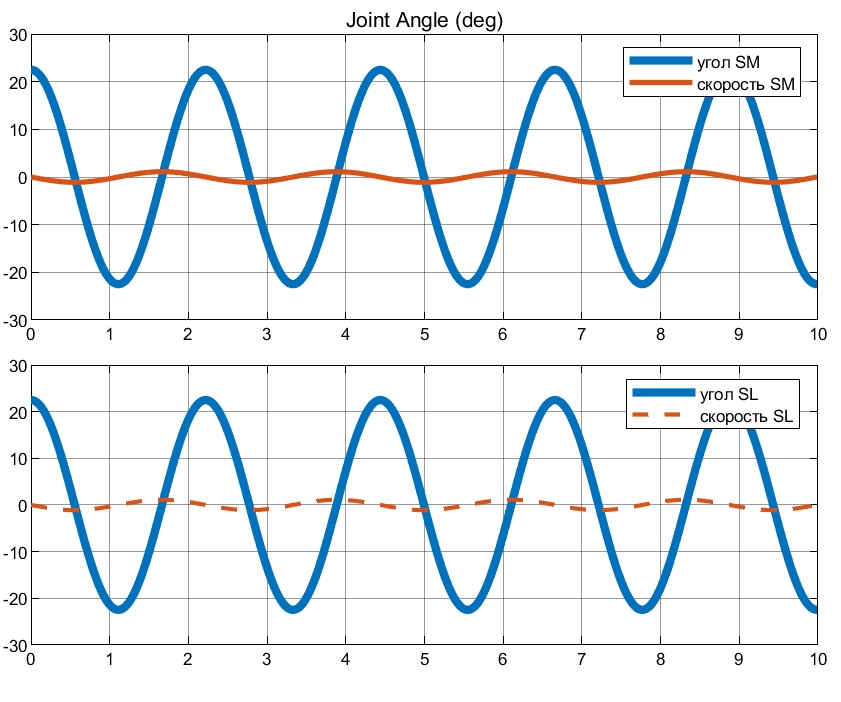
\includegraphics[width=0.7\linewidth]{k1}
		\caption{Зависимость скорости и координаты маятника от времени}
		\label{fig:k1}
	\end{figure}
	\begin{figure}[H]
		\centering
		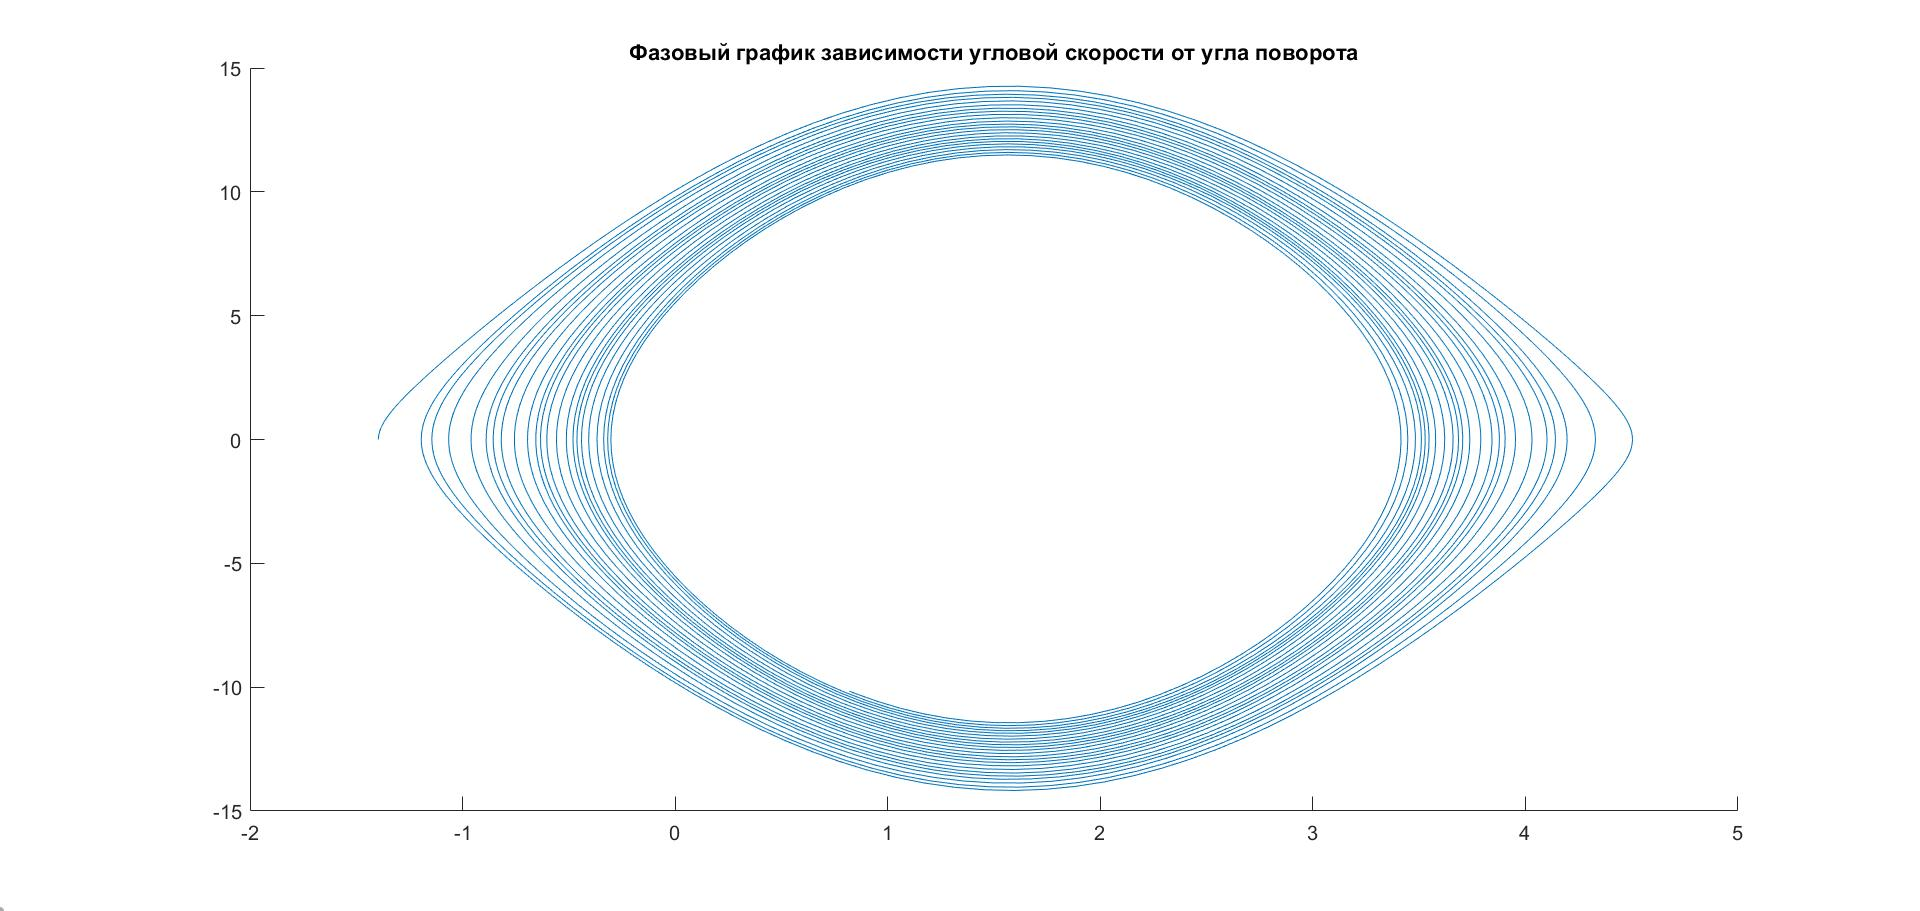
\includegraphics[width=0.7\linewidth]{phase1}
		\caption{Фазовый график зависимости угловой скорости от угла поворота, $\alpha = 0$}
		\label{fig:phase1}
	\end{figure}
	Моделирование свободных колебаний с трением:
	\begin{figure}[H]
		\centering
		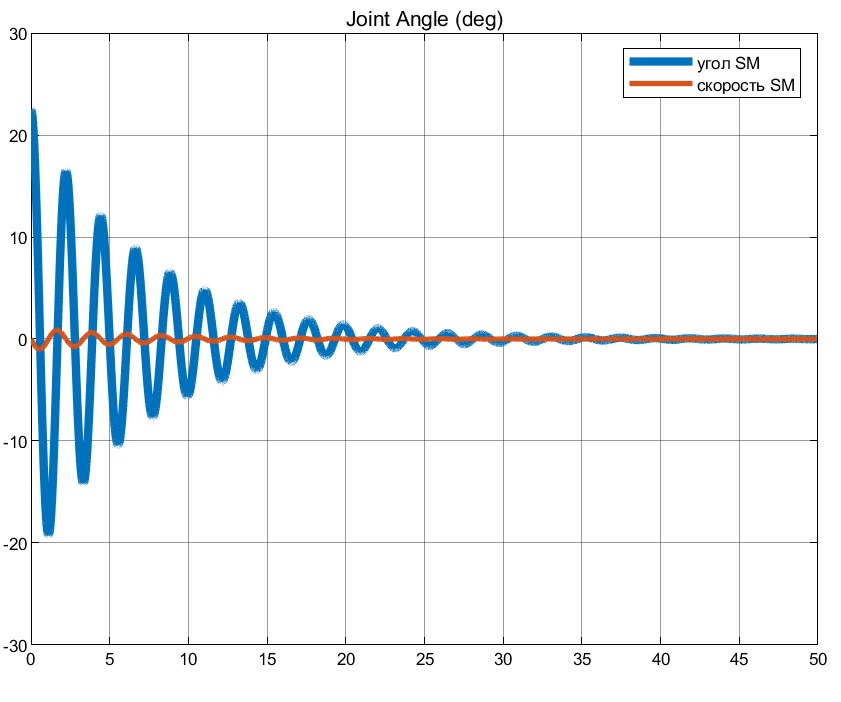
\includegraphics[width=0.7\linewidth]{k2}
		\caption{Зависимость координатыи скорости от времени, $b = 8*10^-5$}
		\label{fig:k2}
	\end{figure}
	\begin{figure}[H]
		\centering
		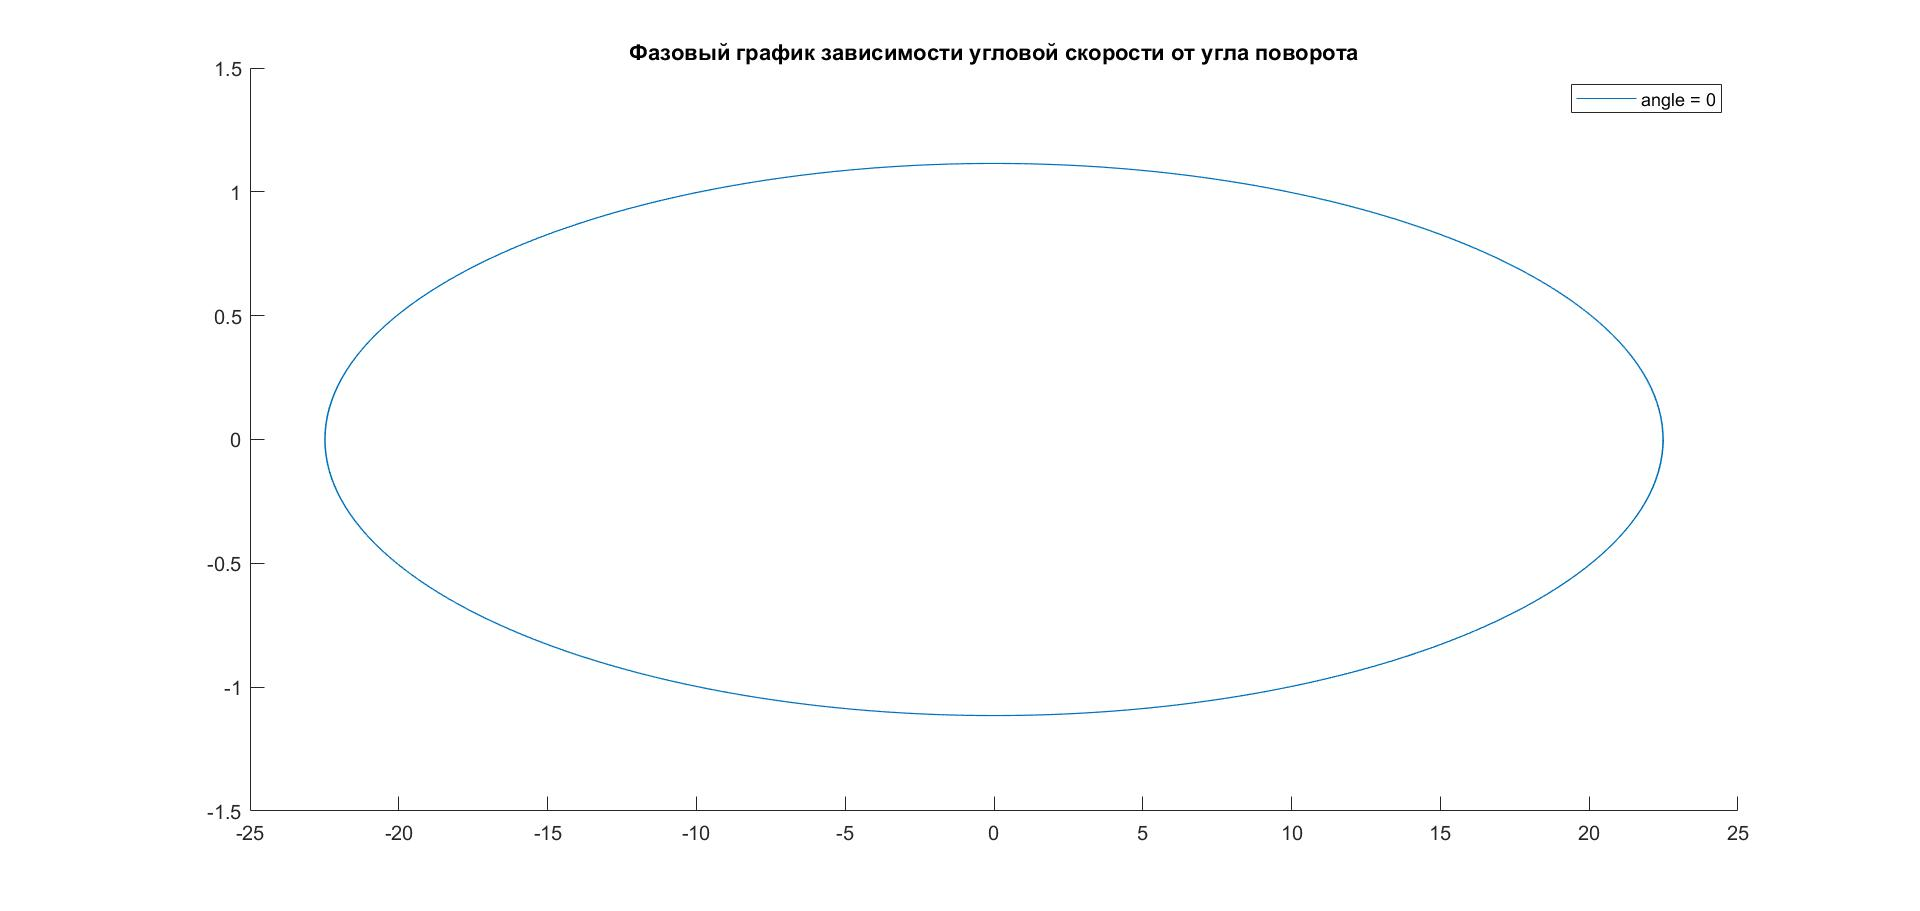
\includegraphics[width=0.7\linewidth]{phase2}
		\caption{Фазовый график зависимости угловой скорости от угла при свободных колебаниях с трением, $b = 8*10^-5$}
		\label{fig:phase2}
	\end{figure}
	Моделирование вынужденных колебаний.\\
	Добавлена периодическая сила с амплитудой 0.06.
	\begin{figure}[H]
		\centering
		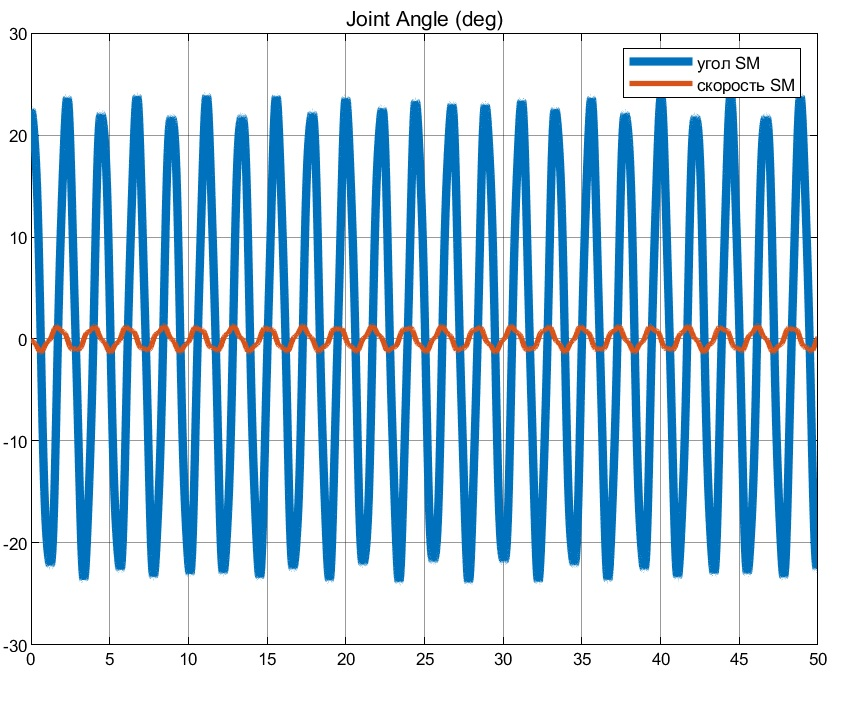
\includegraphics[width=0.7\linewidth]{k3}
		\caption{Зависимость координаты и скорости от времени для вынужденных колебаний, $A =0.06$, $\omega = 10$}
		\label{fig:k3}
	\end{figure}
	\begin{figure}[H]
		\centering
		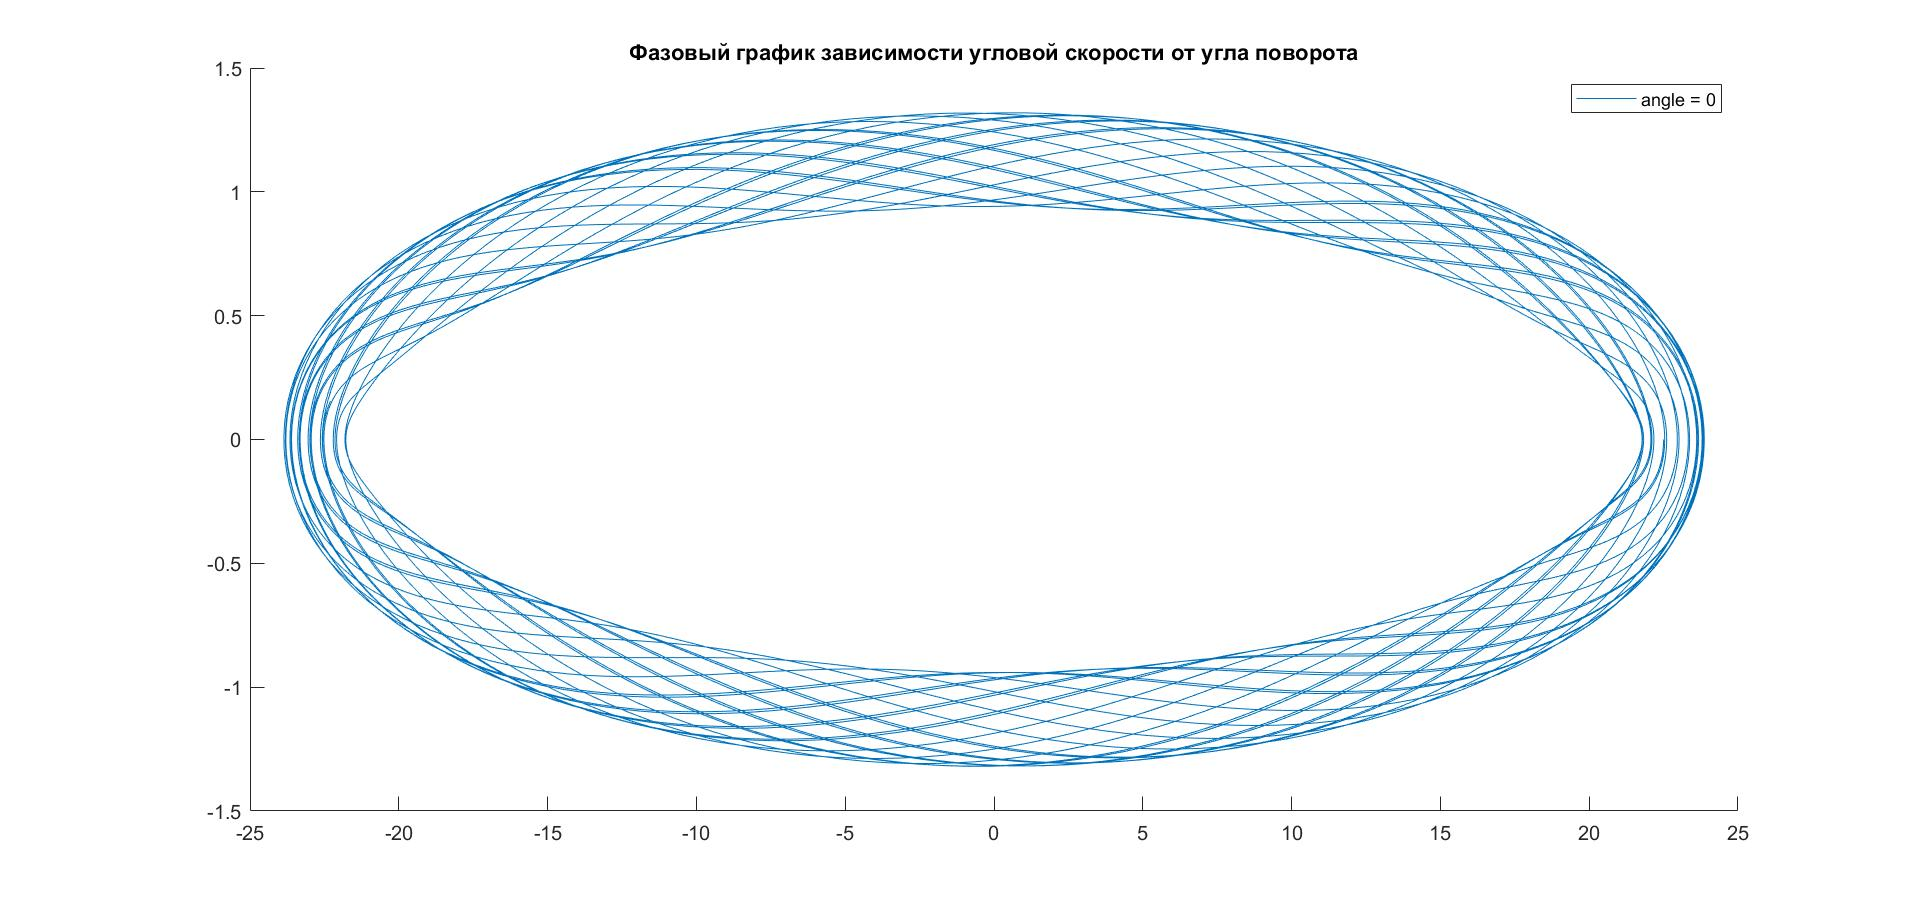
\includegraphics[width=0.7\linewidth]{phase3}
		\caption{Фазовый график для вынужденных колебаний}
		\label{fig:phase3}
	\end{figure}
	\subsection*{Физический маятник}
	Для моделирования была использована блок-схема из 6-го задания
	\begin{figure}[H]
		\centering
		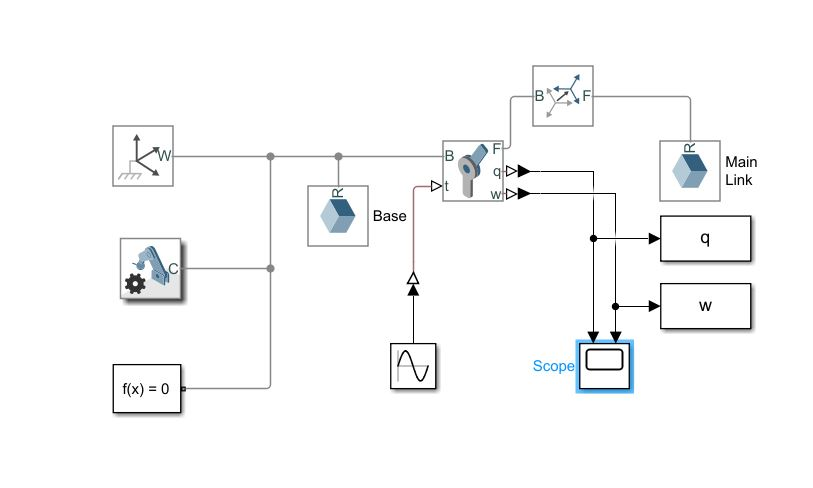
\includegraphics[width=0.7\linewidth]{model}
		\caption{Блок-схема модели физического матника}
		\label{fig:model}
	\end{figure}
	Моделирование свободных колебаний:
	\begin{figure}[H]
		\centering
		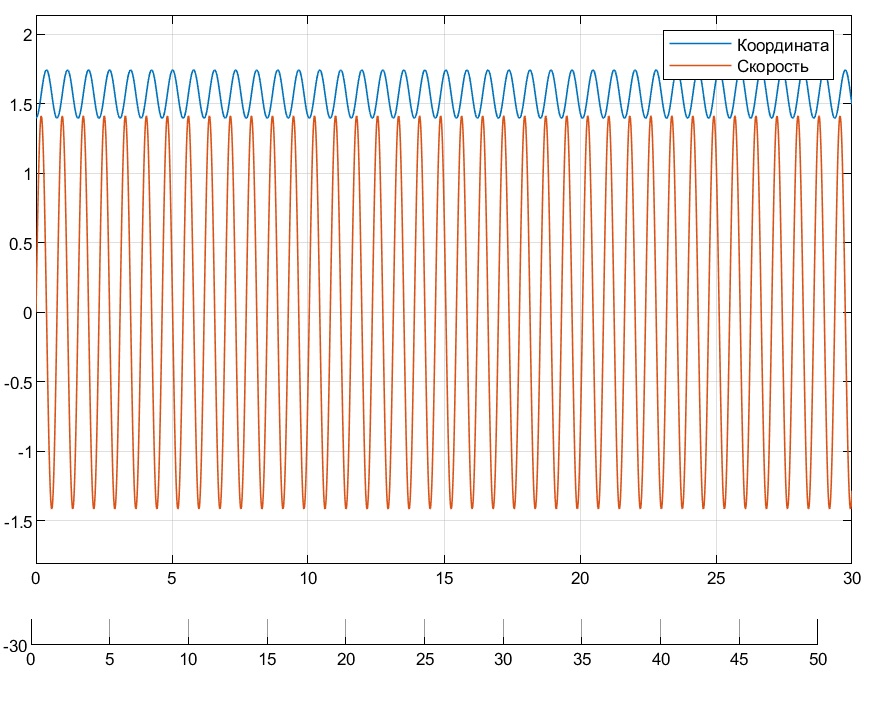
\includegraphics[width=0.7\linewidth]{phys1}
		\caption{Зависимость скорости и координаты от времени}
		\label{fig:phys1}
	\end{figure}
	\begin{figure}[H]
		\centering
		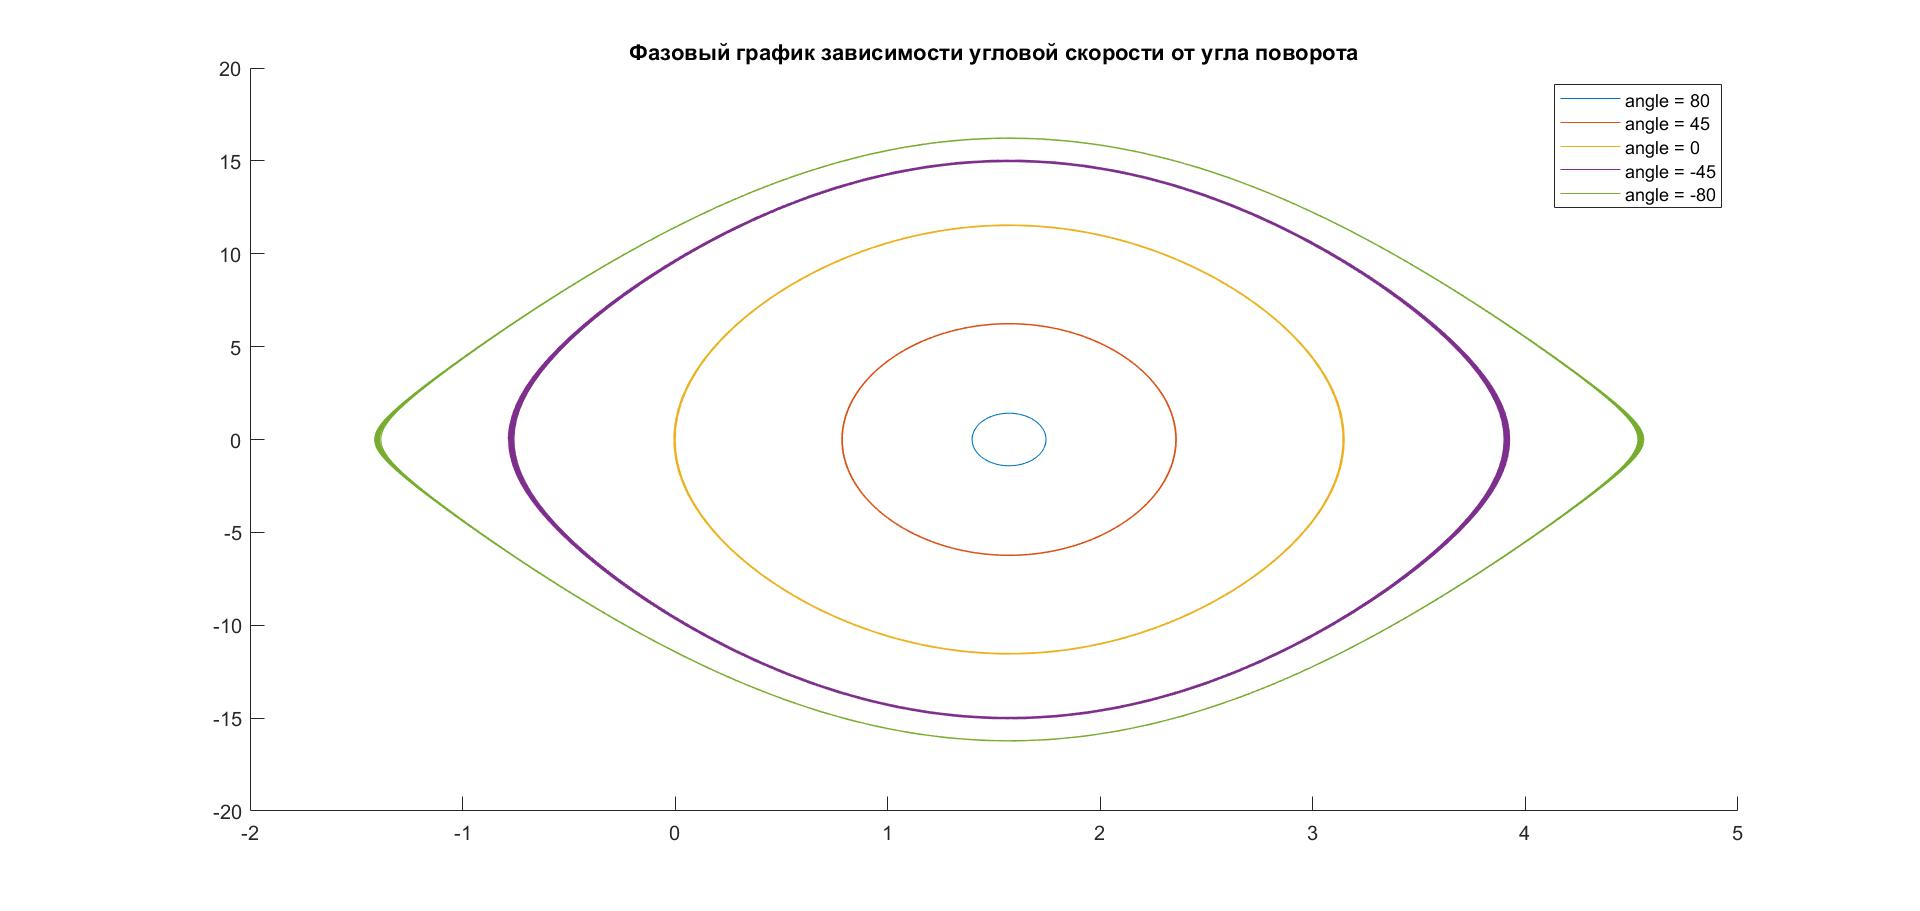
\includegraphics[width=1\linewidth]{pphase1}
		\caption{Фазовый график для значений угла 80, -45, 0, 45, 80 градусов}
		\label{fig:pphase1}
	\end{figure}
	Моделирование свободных колебаний с трением, $b=8*10^-5$
	\begin{figure}[H]
		\centering
		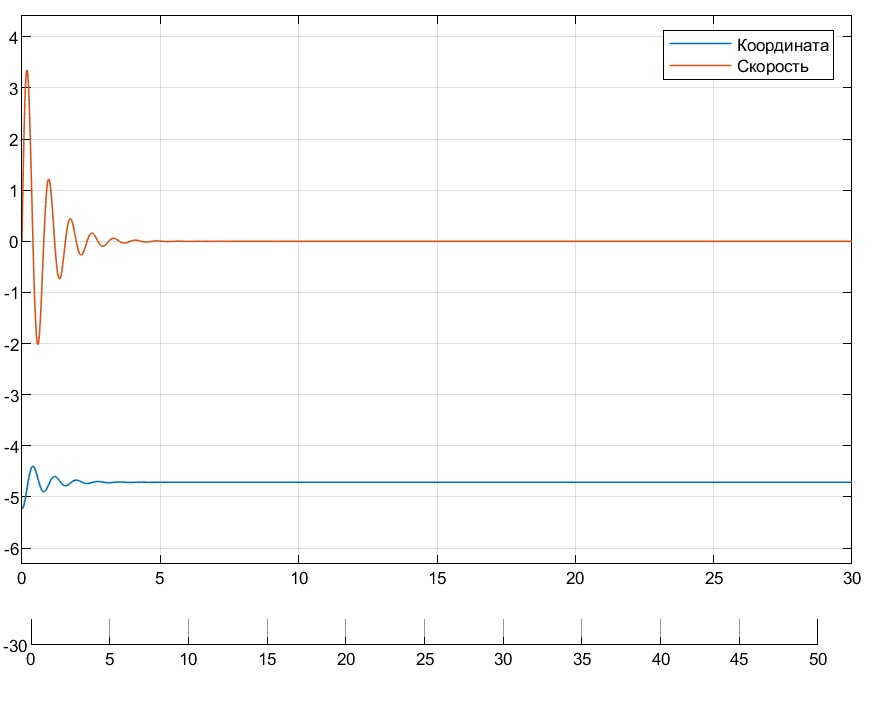
\includegraphics[width=0.7\linewidth]{zatuch}
		\caption{Затухающие колебания, коэффициент трения $b = 8*10^-5$}
		\label{fig:zatuch}
	\end{figure}
	\begin{figure}[H]
		\centering
		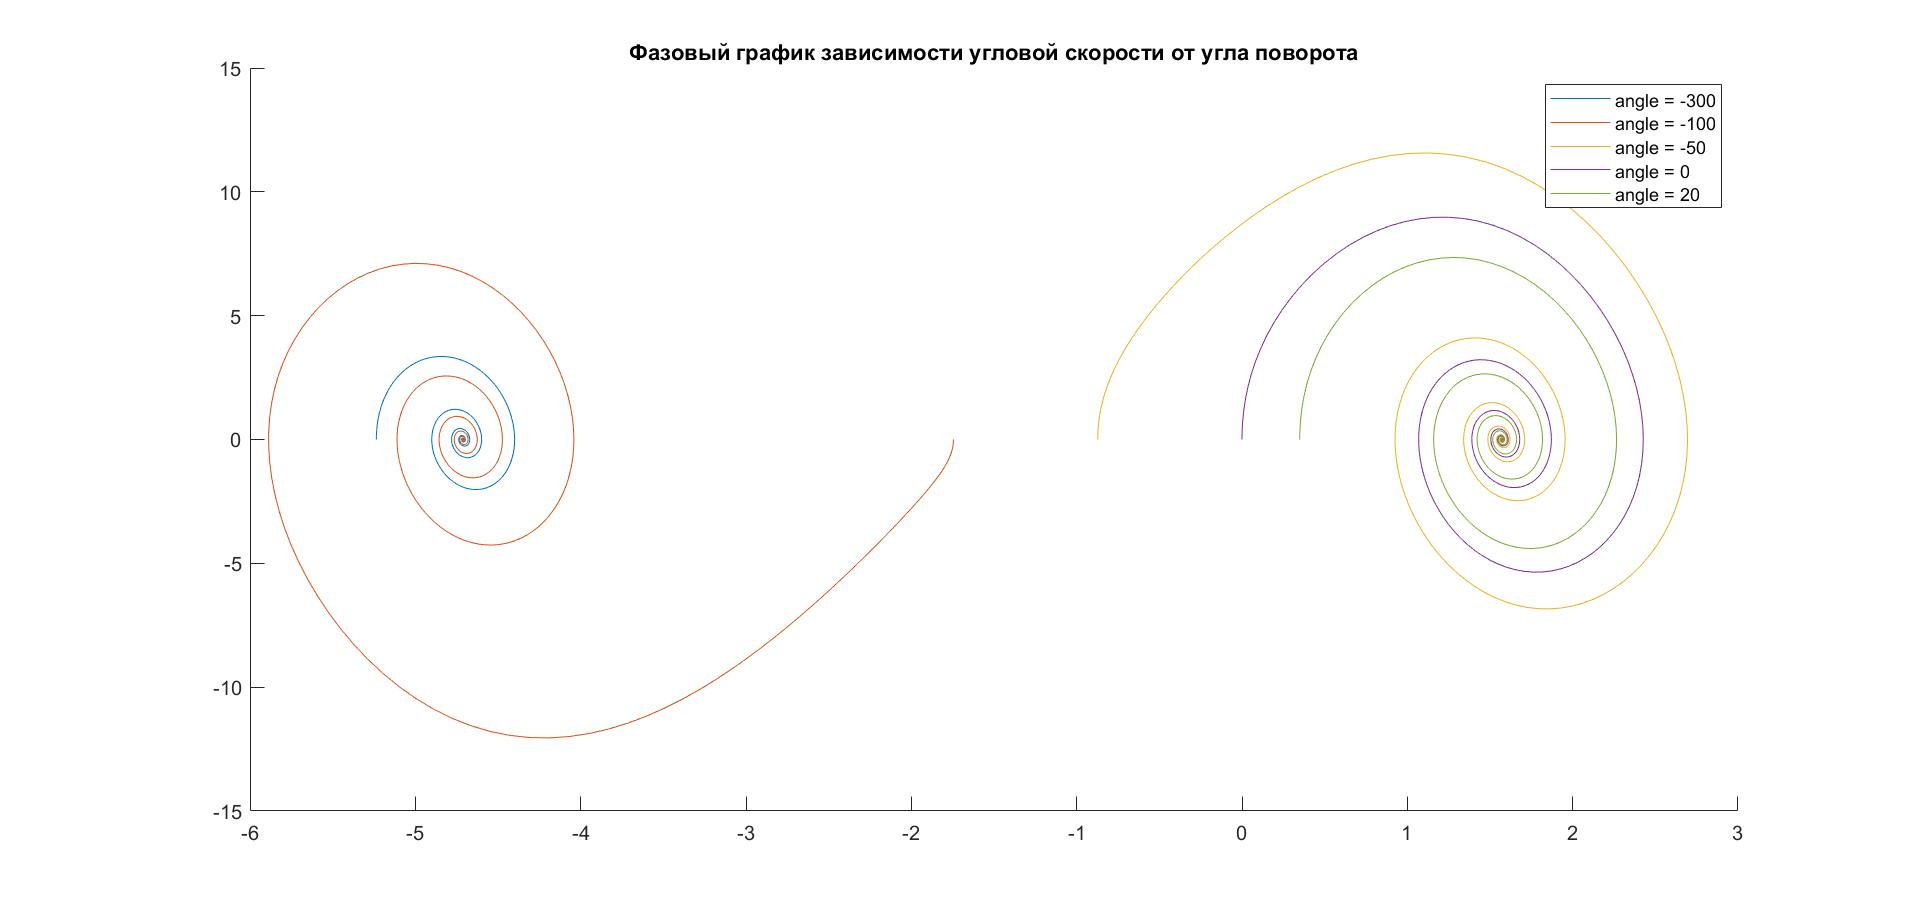
\includegraphics[width=0.7\linewidth]{pphase2}
		\caption{Фазовый график для углов -300, -100, -50, 0, 20 градусов}
		\label{fig:pphase2}
	\end{figure}
	Моделрование вынужденных колебаний, амплитуда силы $A = 0.02$, $\omega = 1$:
	\begin{figure}[H]
		\centering
		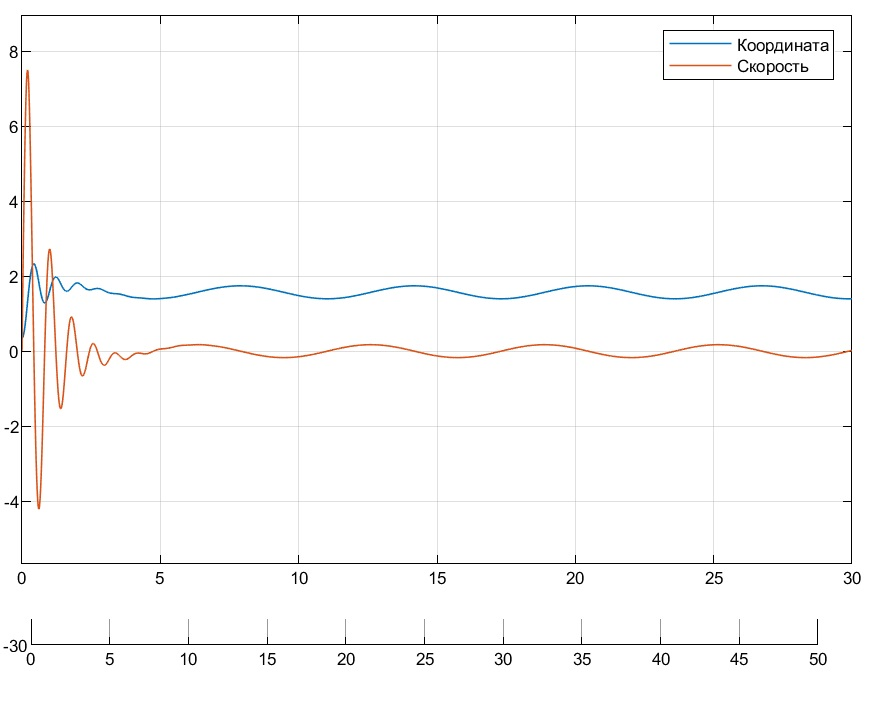
\includegraphics[width=0.7\linewidth]{vinuzhd}
		\caption{Зависимость скорости и ускорения от времени для вынужденных колебаний, $\alpha = 0$}
		\label{fig:vinuzhd}
	\end{figure}
	\begin{figure}[H]
		\centering
		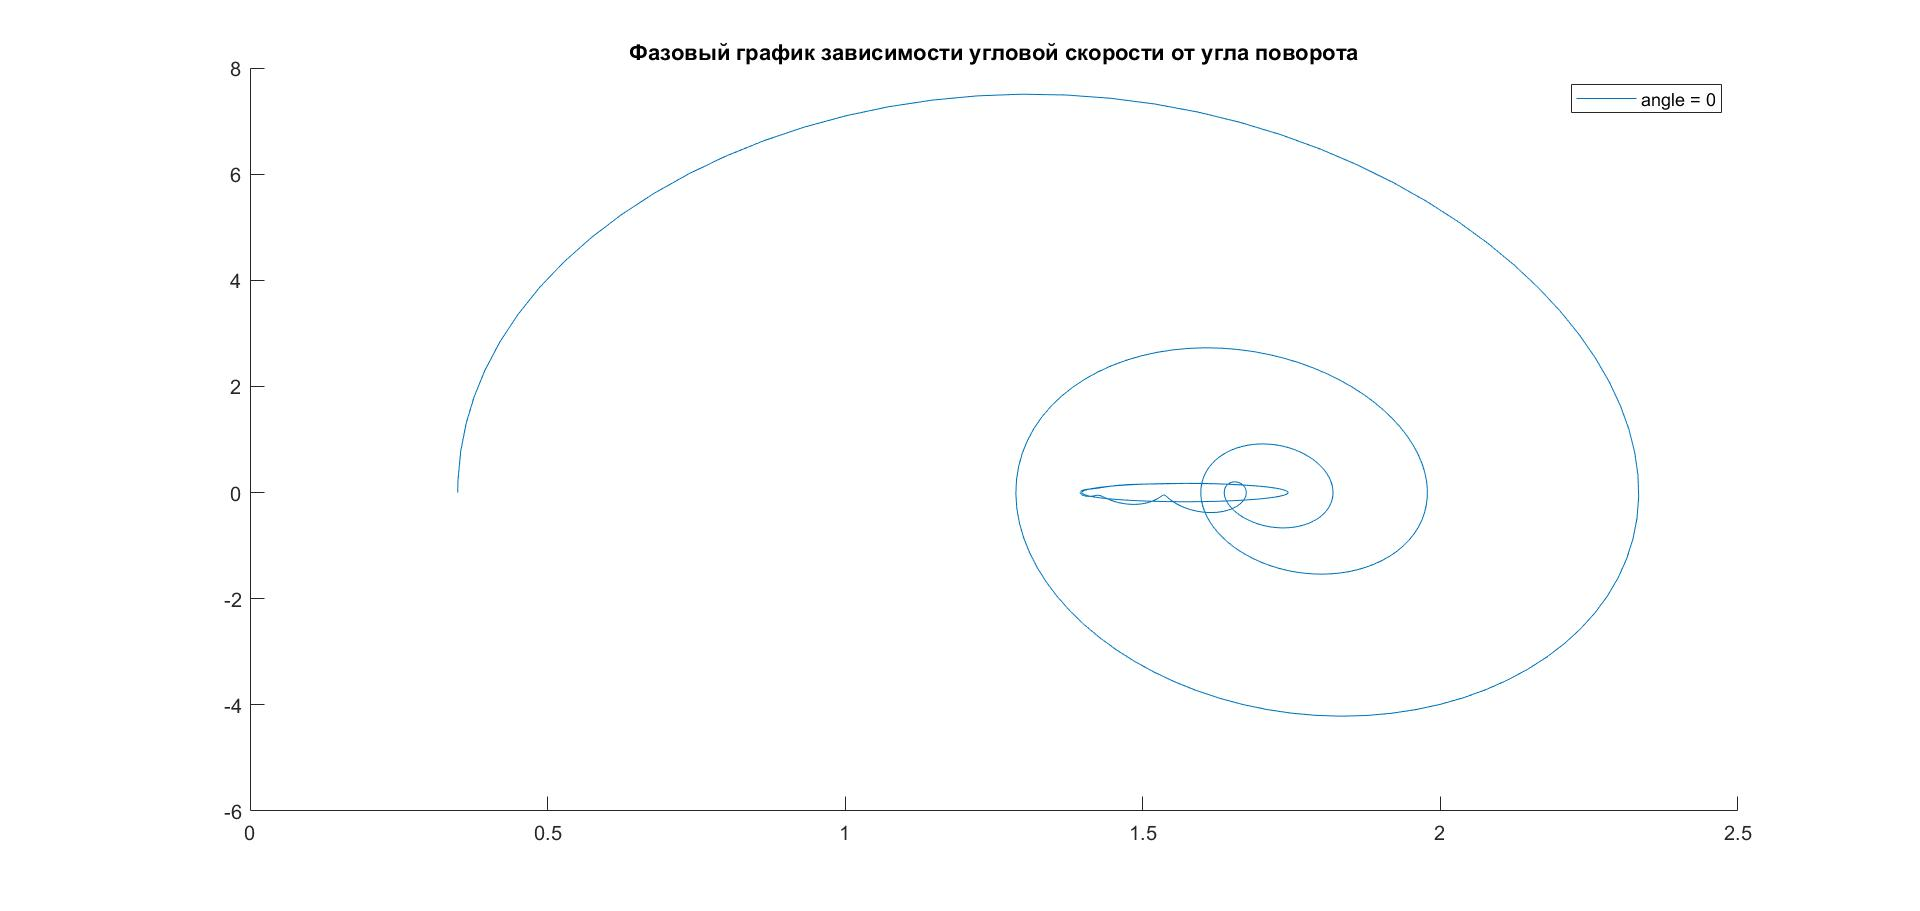
\includegraphics[width=1\linewidth]{pphase3}
		\caption{Фазовый график для вынужденных колебаний; отчетливо видно, что в конце траектории фазовый график приближен к фазовому графику для свободных колебаний при малых углах отклонения}
		\label{fig:pphase3}
	\end{figure}
	
	
\end{document}